\documentclass[english,compress]{beamer}
\usepackage[utf8]{inputenc}
\setcounter{secnumdepth}{3}
\setcounter{tocdepth}{3}
\usepackage{amsmath}
\usepackage{color}
\usepackage{amssymb}
\usepackage{esint}
\usepackage{comment}
\usepackage{listings}
\usepackage{colortbl}
\usepackage{babel}
\usepackage{wasysym}

\definecolor{green}{RGB}{0, 180, 0}
\definecolor{red}{RGB}{180, 0, 0}
\colorlet{grellow}{green!50!yellow}
\colorlet{codeback}{gray!20}

\usepackage{multimedia}

\usepackage{tikz}
\usetikzlibrary{calc}
\usetikzlibrary{positioning}
\usetikzlibrary{fadings}
\usetikzlibrary{chains}
\usetikzlibrary{scopes}
\usetikzlibrary{shadows}
\usetikzlibrary{snakes}
\usetikzlibrary{shapes.misc}
\usetikzlibrary{shapes.symbols}
\usetikzlibrary{fit}
\usetikzlibrary{shapes.arrows}
\usetikzlibrary{shapes.geometric}
\usetikzlibrary{shapes.callouts}

\pgfdeclarelayer{background}
\pgfdeclarelayer{foreground}
\pgfsetlayers{background,main,foreground}

\tikzstyle{every picture}+=[remember picture]

\def\allimgcredits{}
\makeatletter
\def\addimgcredit#1{\g@addto@macro\allimgcredits{\item #1}}
\makeatother
\def\imagecreditslide{
  \begin{frame}[shrink,label=image-credits]{Image Credits}
    \begin{itemize}
      \allimgcredits
    \end{itemize}
  \end{frame}
}

\def\gatheredappendix{}
\makeatletter
\long\def\addtoappendix#1{
  \g@addto@macro\gatheredappendix{#1}
}
\makeatother

\newcommand{\cc}{\raisebox{-0.75ex}{\includegraphics[height=3ex]{cc.pdf}}}

\newcommand{\D}{\mathsf{D}}
\newcommand{\mathd}{\,\mathsf{d}}

\newcommand{\avg}[1]{\{#1\}}
\newcommand{\jump}[1]{\left\llbracket#1\right\rrbracket}

\newcommand{\questionframe}[1]{
  \begin{frame}{Questions?}
    \begin{center}
    \textbf{\Huge ?}
    \par#1
    \end{center}
  \end{frame}
}

\lstset{
  language=Python,
  showstringspaces=false,
  basicstyle=\small,
  stringstyle=\color{blue},
  columns=flexible,
  emph={[2]starcluster,paramiko,boto},
  emphstyle={[2]\color{red}},
  backgroundcolor=\color{codeback},
  frame=single,
  framerule=0pt,
  framesep=1.5pt,
  rangebeginprefix=//\ ,
  rangeendprefix=//\ ,
  includerangemarker=false,
  }

\def\mylogotext{\pgfuseimage{brown-logo}\hspace*{0.3cm}}
\newcommand{\logoenable}{\logo{\mylogotext}}
\newcommand{\logodisable}{ \logo{} }
\newenvironment{nologo}{\logodisable}{\logoenable}

\newcommand{\symball}[2]{
  \begin{tikzpicture}[baseline=-0.7ex]
    \shadedraw [shading=ball,ball color=#1,use as bounding box] 
      circle (1ex) node at (0.7ex,0) [minimum width=0.7ex] {};

    \node [text=white,font=\bfseries] {#2};
  \end{tikzpicture}}
\newcommand{\plusball}{\symball{green}{{\small +}}}
\newcommand{\okball}{\symball{orange}{o}}
\newcommand{\minusball}{\symball{red}{-}}

\let\epsilon=\varepsilon
\let\phi=\varphi

\newcommand{\subitem}[1]{\begin{itemize}\item #1 \end{itemize}}

\nonstopmode

\usetheme[compress]{Berlin}
\usecolortheme{mit}

\AtBeginSection[] {
  \begin{frame}<beamer>
  \frametitle{Outline}
  \tableofcontents[sectionstyle=show/shaded,subsectionstyle=show/show/hide]
\end{frame}
}

\definecolor{green}{RGB}{0, 180, 0}
\definecolor{red}{RGB}{180, 0, 0}
\colorlet{grellow}{green!50!yellow}
\colorlet{codeback}{gray!20}

\DeclareMathOperator{\argmin}{argmin}
\DeclareMathOperator{\argmax}{argmax}

\lstset{
  language=Python,
  }

\newenvironment{changemargin}[2]{%
  \begin{list}{}{%
    \setlength{\topsep}{0pt}%
    \setlength{\leftmargin}{#1}%
    \setlength{\rightmargin}{#2}%
    \setlength{\listparindent}{\parindent}%
    \setlength{\itemindent}{\parindent}%
    \setlength{\parsep}{\parskip}%
  }%
  \item[]}{\end{list}}



\batchmode

\usepackage{amsmath,amssymb,enumerate,epsfig,bbm,calc,color,ifthen,capt-of}

\usetheme{Berlin}
\usecolortheme{mit}

\title{StarCluster - NumPy/SciPy Computing on Amazon's Elastic Compute Cloud (EC2)} 
\author{Justin Riley}
\institute[Massachusetts Institute of Technology] % (optional, but mostly needed)
{
  Software Tools for Academics and Researchers\\
  Office of Educational Innovation and Technology\\
  Massachusetts Institute of Technology}
\date[SciPy 2010]{SciPy 2010}
\pgfdeclareimage[height=0.5cm]{mit-logo}{mit-logo.pdf}
\logo{\pgfuseimage{mit-logo}\hspace*{0.3cm}}

\AtBeginSection[]
{
  \begin{frame}<beamer>
    \frametitle{Outline}
    \tableofcontents[currentsection]
  \end{frame}
}
\beamerdefaultoverlayspecification{<+->}
% -----------------------------------------------------------------------------
\begin{document}
% -----------------------------------------------------------------------------

\frame{\titlepage}

\section[Outline]{}
\begin{frame}{Outline}
  \tableofcontents
\end{frame}

% -----------------------------------------------------------------------------
\section{Introduction}
\subsection{STAR Group}
\begin{frame}{Software Tools for Academics and Researchers}
	STAR Group
\end{frame}

\subsection{StarCluster Motivations}
\begin{frame}{StarHPC\dots}
\begin{figure}
\begin{center}
\hspace*{-1.2cm}
\begin{tikzpicture}
\node (laptop) [label=below:User] {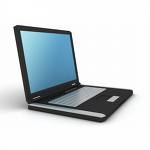
\includegraphics[width=1in]{laptop.png}};
\node (cloud) [right=of laptop, label=below:EC2] {
\includegraphics[width=1in]{cloud.png}};
\node (screenshot) [right=of cloud, label=below:Virtual Desktop] {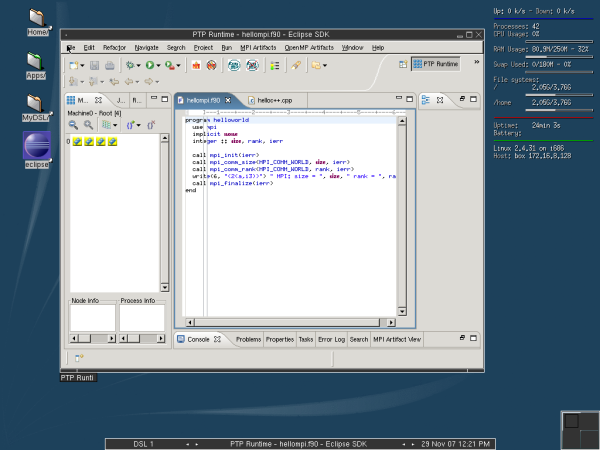
\includegraphics[width=2in]{hpc-screenshot.png}};
\draw [->,thick] (laptop) to (cloud)
  node [pos=0.5,above=0.2cm] {SSH};
\draw [->,thick] (cloud) to (screenshot)
  node [pos=0.5,above=0.2cm] {VNC};
\end{tikzpicture}
\end{center}
\caption{\label{fig:SRD} StarHPC Overview}
\end{figure}
\end{frame}

\begin{frame}{StarMolSim\dots}
	TODO
\end{frame}

% -----------------------------------------------------------------------------

% -----------------------------------------------------------------------------
\section{Amazon EC2 Basics}
\subsection{Amazon EC2 Instance Types}
\begin{frame}{Elastic Compute Cloud Overview}
\begin{itemize}
  \item Infrastructure as a Service (IaaS)
  \item Up to 20 virtual machines by default
  \item Full root access
  \item Pay only for what you use
\end{itemize}
\end{frame}

\begin{frame}{Simple Storage Solution (S3)}
  Simple Storage Solution
\end{frame}

\begin{frame}{Elastic Block Storage}
  Elastic Block Storage Devices
\end{frame}


\begin{nologo}
\begin{frame}{Standard Instances}
\begin{definition}
1 Compute Unit (CU) = 1.0-1.2 GHz 2007 Opteron or 2007 Xeon processor.
\end{definition}
\begin{center}
	\small
	\begin{tabular}{ l  l  l  l  l  l  l }
	  Instance & Arch & CPU (CU) & RAM & Storage & I/O & Cost/hr \\\hline \\ [-1.5ex]
	  Small     & 32bit & 1 (x1) & 1.7GB & 160GB & Moderate & \$0.085 \\ [1.5ex]
	  Large     & 64bit & 2 (x2) & 7.5GB & 860GB & High & \$0.34 \\ [1.5ex]
	  X-Large   & 64bit & 2 (x4) & 15GB & 1.69TB & High & \$0.68 \\ [1.5ex]
	\end{tabular}
\end{center}
\end{frame}

\begin{frame}{High-Memory Instances}
\begin{definition}
1 Compute Unit (CU) = 1.0-1.2 GHz 2007 Opteron or 2007 Xeon processor.
\end{definition}
\begin{center}
	\small
	\begin{tabular}{ l  l  l  l  l  l  l }
	  Instance & Arch & CPU (CU) & RAM & Storage & I/O & Cost/hr \\\hline \\ [-1.5ex]
	  X-Large     & 64bit & 3.25 (x2) & 17.1GB & 420GB & Moderate & \$0.50 \\ [1.5ex]
	  2X-Large    & 64bit & 3.25 (x4) & 34.2GB & 850GB & High & \$1.20 \\ [1.5ex]
	  4X-Large    & 64bit & 3.25 (x8) & 68.4GB & 1.69TB & High & \$2.40 \\ [1.5ex]
	\end{tabular}
\end{center}
\end{frame}

\begin{frame}{High-CPU Instances}
\begin{definition}
1 Compute Unit (CU) = 1.0-1.2 GHz 2007 Opteron or 2007 Xeon processor.
\end{definition}
\begin{center}
	\small
	\begin{tabular}{ l  l  l  l  l  l  l }
	  Instance & Arch & CPU (CU) & RAM & Storage & I/O & Cost/hr \\\hline \\ [-1.5ex]
	  Medium   & 32bit & 2.5 (x2) & 1.7GB & 160GB & Moderate & \$0.17 \\ [1.5ex]
	  X-Large  & 64bit & 2.5 (x8) & 15GB & 1.69TB & High & \$0.68 \\ [1.5ex]
	\end{tabular}
\end{center}
\end{frame}
\end{nologo}

\begin{frame}{AWS Funding Opportunities}
	\begin{itemize}
		\item Teaching Grants for educators using AWS in courses
		\item Research Grants for academic researchers using AWS in their work
		\item Project Grants for student organizations pursuing entrepreneurial endeavors
	\end{itemize}
\end{frame}

\questionframe{}
% -----------------------------------------------------------------------------

% -----------------------------------------------------------------------------
\section{StarCluster Overview}
\subsection{Features}
\begin{frame}{About}
	\newcolumntype{V}{>{\centering\arraybackslash} m{.2\linewidth} }
	\begin{tabular}{ V m{8cm} }
	\centering
	
\includegraphics[scale=0.50]{logo.png} & StarCluster allows anyone to create their own scientific computing cluster on Amazon's Elastic Compute Cloud (EC2) \\
	\end{tabular}

	\vspace{1cm}

	Dependencies:
	\begin{itemize}
		\item Registered and fully configured EC2 account
		\item Python 2.4+
		\item Boto (AWS library for Python)
		\item Paramiko (SSH library for Python)
	\end{itemize}
\end{frame}

\begin{frame}{StarCluster Features}
  \begin{itemize}
    \item Simple configuration file for defining cluster settings
    \item Single "start" command to create a cluster
    \item "stop" command to terminate a cluster and stop paying for it
    \item Automatic configuration of: 
    \item Network File System (/home and all EBS volumes)
    \item Sun Grid Engine
    \item Passwordless-ssh
    \item OpenMPI, etc
  \end{itemize}
\end{frame}

\begin{frame}{NumPy/SciPy on StarCluster}
	TODO
\end{frame}

\begin{frame}{Sun Grid Engine (open-source edition)}
	TODO
\end{frame}

\begin{frame}{Elastic Block Storage}
	TODO
\end{frame}

\subsection{Plugins}
\begin{nologo}
\begin{frame}[fragile]{StarCluster Plugin System}
  \lstinputlisting[numbers=left, basicstyle=\footnotesize]{ubuntu-plugin.py}
  %\vspace*{0.5cm}
  %[This is \texttt{examples/demo.py} in the starcluster distribution]
\end{frame}
\end{nologo}

\questionframe{}
% -----------------------------------------------------------------------------

% -----------------------------------------------------------------------------
\section{Conclusions}
\subsection{Where can I learn more?}
\begin{frame}{Questions and Answers}
  Want to know more?
  \begin{itemize}
    \item Homepage: \url{http://web.mit.edu/starcluster}.
    \item Code: \url{http://github.com/jtriley/StarCluster}.
    \item Mailing list: \url{http://mailman.mit.edu}.
    \item Software Tools for Academics and Researchers \url{http://web.mit.edu/star}.
  \end{itemize}
\end{frame}

% -----------------------------------------------------------------------------
\end{document}
